\section{Design Science Research}
\label{sec:dsr-approach}

Unlike traditional natural sciences that seek to understand reality (positivism) or social sciences that seek to interpret it (interpretivism), Design Science is rooted in the pragmatic epistemology. Its fundamental goal is to change reality through the creation of innovative artifacts.

As defined by \citeonline{simon_1969} and consolidated by \citeonline{hevner_2004}, DSR involves the rigorous process of designing artifacts to solve observed problems, make research contributions, and evaluate the designs. In the context of this thesis, the primary artifact is PANOPTES, a reference architecture for observability.

According to the classification by \citeonline{vaishnavi_2008}, the desired outputs of DSR are classified by level of abstraction as described in table \ref{tab:dsr-outputs}.

\input{chapters/05.methodology/tables/dsr-outputs.tex}

The artifacts produced in this research are of two types:
\begin{itemize}
    \item \textbf{Architecture:} A high-level structural framework defining components (Metrics, Logs, Traces) and their relationships.
    \item \textbf{Instantiation:} A concrete implementation (Infrastructure as Code) that operationalizes the architecture in a working environment.
\end{itemize}

\subsection{Research Cycles}
\label{subsec:research-cycles}

Following the framework proposed by \citeonline{hevner_2004}, this research operates across three cycles as depicted in figure \ref{fig:dsr-cycles} :

\begin{figure}[ht]
    \centering
    \caption{Design science research cycles}
    \label{fig:dsr-cycles}
    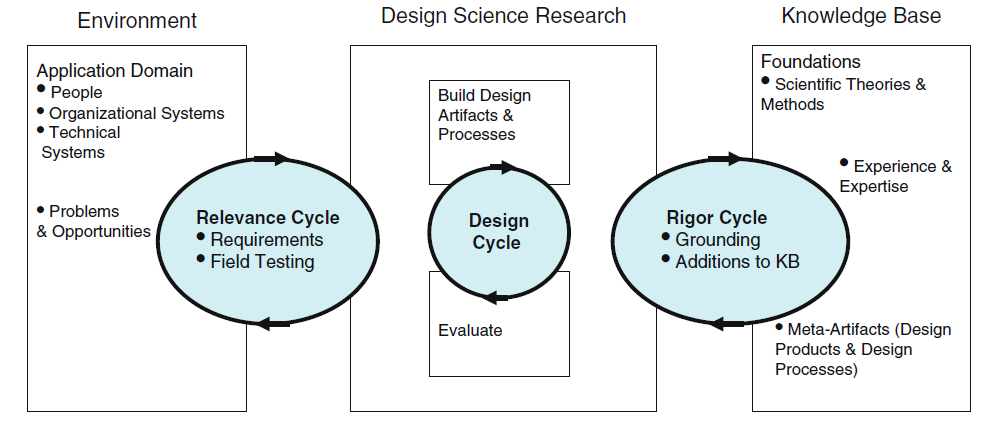
\includegraphics[width=1.0\linewidth]{images/methodology/hevner-dsr-cycles.png}
    \par\medskip\ABNTEXfontereduzida\selectfont\textbf{Source:} \cite{hevner_2004} \par\medskip
\end{figure}

\subsection{Research Cycles Instantiation}
\label{subsec:cycles-instantiation}

To operationalize the Design Science Research (DSR) framework, we instantiated the research cycles defined by \cite{hevner_2007} and \cite{dresch_2015}, moving beyond mere artifact construction toward structured \textit{design theorizing}. Figure \ref{fig:panoptes-cycles} illustrates the integration of the Knowledge Base with the iterative research cycles.

\begin{figure}[ht]
    \centering
    \caption{Instantiation of DSR Cycles for PANOPTES Research}
    \label{fig:panoptes-cycles}
    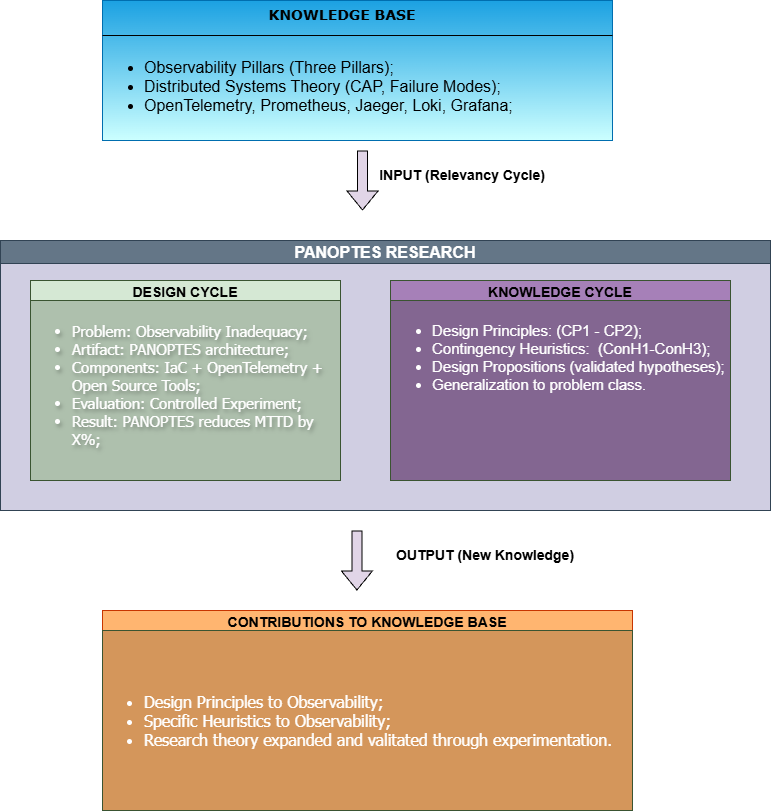
\includegraphics[width=1.0\textwidth]{images/methodology/design-cycle.png}
    \par\medskip
    \small\textbf{Source:} Author (2026), adapted from \cite{dresch_2015} and \cite{hevner_2007}.
\end{figure}

The research process is structured into three iterative cycles:

\begin{enumerate}
    \item \textbf{Relevance Cycle:} Bridges the research to the cloud-native environment. We identified the problem of ``observability fragmentation'' as a \textit{wicked problem}, establishing requirements based on practitioner needs in Chapters \ref{chap:observability} and \ref{chap:cloud-computing}.
    
    \item \textbf{Design Cycle:} This is the core iterative process of building the PANOPTES architecture. We operationalized the design process by defining \textit{Design Principles} (CPs) and \textit{Contingency Heuristics} (ConHs), which prescribe how the artifact should be constructed to meet observability requirements \cite{walls_1992}. This ensures that our Ansible and Helm instantiations (Chapter \ref{chap:experiment-implementation}) are grounded in architectural theory rather than mere \textit{ad hoc} implementation.
    
    \item \textbf{Rigor Cycle:} Connects the design efforts back to the scientific knowledge base. We utilized Control Theory as our \textit{Kernel Theory}, grounding our design decisions in feedback-loop mechanisms common in distributed systems \cite{wieringa_2014}. 
\end{enumerate}

To ensure traceability and generalizability, we mapped classical SRE challenges into formal Design Principles and Contingency Heuristics. These were derived by treating the observability stack as a control system (Sensor $\rightarrow$ Controller $\rightarrow$ Actuator), where the telemetry pipeline acts as the \textit{feedback signal}.

\begin{table}[ht]
\centering
\caption{Mapping SRE Challenges to PANOPTES Research Concepts}
\label{tab:sre-mapping}
\begin{tabularx}{\textwidth}{|l|p{3cm}|X|}
\hline
\textbf{ID} & \textbf{SRE Problem} & \textbf{Formalization (Control Theory Grounding)} \\ \hline
CP1 & RCA and Correlation & \textbf{Principle of Causal Linkage:} Ensures observability signals maintain temporal context for state attribution. \\ \hline
CP2 & Single Pane of Glass & \textbf{Principle of Unified State Representation:} Integration of telemetry signals via standardized schemas (OTLP). \\ \hline
ConH1 & Config/K8s Complexity & \textbf{Heuristic of Declarative Control:} Use operators to automate state synchronization between K8s and tools. \\ \hline
ConH2 & IaC Change Tracking & \textbf{Heuristic of Configuration Drift:} Link state changes to infrastructure commits to minimize external disturbances. \\ \hline
ConH3 & Load Control & \textbf{Heuristic of Adaptive Feedback:} Dynamic adjustment of sampling rates based on resource consumption (CPU/Memory). \\ \hline
\end{tabularx}
\par\medskip\ABNTEXfontereduzida\selectfont\textbf{Source:} The Author (2026) \par\medskip
\end{table}

The theoretical foundation of these elements is grounded in Control Theory \cite{wieringa_2014}:
\begin{itemize}
    \item \textbf{Design Principles (CPs):} These define the structural axioms of the system. The \textit{Principle of Causal Linkage} (CP1) grounds observability as the ''sensor'' component, where state attribution is impossible without explicit causal context. Similarly, the \textit{Principle of Unified State Representation} (CP2) leverages \textit{State-Space Representation} to normalize heterogeneous telemetry signals (logs, metrics, traces) into a coherent model.
    
    \item \textbf{Contingency Heuristics (ConHs):} These address the \textit{Treatment Validation} and environmental constraints. The \textit{Heuristic of Declarative Control} (ConH1) minimizes the "control delay" in closed-loop systems by favoring automated reconciliation over manual intervention. The \textit{Heuristic of Configuration Drift} (ConH2) treats configuration changes as external disturbances to be rejected, while the \textit{Heuristic of Adaptive Feedback} (ConH3) applies the \textit{Observer Effect} rationale: in high-load scenarios, the system must dynamically adjust signal resolution (sampling) to prevent the observability stack from destabilizing the primary system it intends to monitor.
\end{itemize}

This grounding allows the PANOPTES system to detect disturbances (e.g., latency or resource saturation) and correlate them with state changes tracked via IaC, fulfilling the rigor requirement of the DSR framework.

\subsection{Synthesis of Design Knowledge}
\label{subsec:design-knowledge}

One of the primary goals of DSR is to generate knowledge that extends beyond the specific instantiation of the artifact. According to \citeonline{gregor_2013}, this knowledge is crystallized in the form of Design Principles and Contingency Heuristics.

In this thesis, these elements are defined as follows:

\begin{itemize}
    \item \textbf{Design Principles:} Fundamental rules that guide the construction of the artifact to ensure it addresses the research problem. These are derived from the Knowledge Base (e.g., Control Theory, Distributed Systems Patterns) during the Rigor Cycle.
    \item \textbf{Contingency Heuristics:} Context-aware rules of thumb (e.g., ``If condition $X$ occurs in the cluster, apply strategy $Y$'') that guide practitioners in adapting the architecture to specific scenarios.
\end{itemize}

The validity of these principles is established through the Design Cycle (construction) and verified by the Evaluation Step (Controlled Experiment). The formalized principles and heuristics are presented as the final contribution of the Knowledge Cycle in Chapter \ref{chap:conclusion}.